\documentclass[11pt]{article}
\usepackage[margin=1in]{geometry}
\usepackage[T1]{fontenc}
\usepackage{lmodern,microtype,amsmath,amssymb,amsthm,booktabs,graphicx,natbib}
\usepackage[colorlinks=true,allcolors=blue]{hyperref}
\hypersetup{pdftitle={Regression Calibration as a Baseline for Machine-Learned Covariates}}
\usepackage{setspace}
\setstretch{1.15}
\newtheorem{proposition}{Proposition}
\newcommand{\E}{\mathbb{E}}
\newcommand{\SimulationReps}{400}
\newcommand{\InferenceReps}{400}
\newcommand{\BootstrapDraws}{399}

\newcommand{\SmallMedian}{0.065}
\newcommand{\ValidationMedian}{0.057}
\newcommand{\ExpandedMedian}{0.341}

\title{Regression Calibration as a Baseline\\for Machine-Learned Covariates}
\author{}
\date{October 2026}
\begin{document}
\maketitle
\begin{abstract}
Researchers increasingly use machine-learning predictions as covariates, including controls for confounding. Prediction error can then change the estimated effect of interest. Regression calibration offers an established baseline: use a labeled sample to predict the true covariate from its machine-generated surrogate and the other regression variables. We explain when this procedure identifies a linear model and what can go wrong when calibration must itself be learned. A population projection can suffice without a correct conditional-mean model, but estimated calibration must preserve the residual relationships that identify the downstream coefficients. We connect departures from those relationships to coefficient error, distinguish many calibration predictors from many mismeasured covariates, and separate estimation error from failures of support and transport. Exact examples show how omitting treatment or imposing shrinkage changes confounding adjustment; simulations illustrate these mechanisms. The resulting framework makes regression calibration a transparent benchmark for evaluating methods that use machine-learned covariates.
\end{abstract}

\section{Introduction}
A researcher uses a model to infer a confounder from text, images, or administrative records, then controls for that prediction in a regression. A good prediction need not be a good control. Its errors can leave part of the confounder associated with treatment, changing the estimated treatment effect. The practical question is which correction is justified by the labeled data and the downstream model.

Regression calibration deserves a place among the baselines. It replaces an error-prone covariate with a prediction of its true value conditional on available information. This is an established measurement-error method, not a new solution to machine-learning error \citep{carroll1990,boe2023}. For a linear outcome model, a suitable calibration residual is orthogonal to the regressors used downstream. That fact explains both the attraction of calibration and its requirements. A machine-learning prediction may already satisfy the requirement; an additional calibration step is useful when it does not.

Work on machine-generated regressors has developed corrections tailored to the information available in validation samples \citep{fong2021,battaglia2025}. Prediction-powered inference and design-based approaches use labeled observations to correct downstream estimation \citep{angelopoulos2023,egami2023}; \citet{kluger2025} address imputed covariates and nonuniform sampling explicitly. These methods need not share calibration's outcome exclusion restriction or its target. A procedure for a population regression projection can remain meaningful when a structural linear model fails. Cross-prediction-powered inference concerns reuse of prediction-training observations and should not be conflated with a result specifically about covariate calibration \citep{zrnic2024cross}.

The useful comparison begins with a distinction between population calibration and estimated calibration. At the population level, a linear projection onto a feature span containing the observed downstream regressors can be enough. It need not recover the full conditional mean. In practice, however, a labeled sample must estimate that projection or a more flexible function. Adding predictors can increase estimation variance; shrinkage can alter the required orthogonality; and observations outside the labeled sample's support require extrapolation. If several covariates are mismeasured, their calibrated values may also lack the independent variation needed to identify their separate coefficients.

This note organizes these issues around the residual moments that determine downstream coefficient error. Its contribution is a formulation of the baseline and its failure modes for machine-learned covariates, with explicit implications for confounding adjustment. The calibration identity, two-stage uncertainty correction, and general concerns about predicted regressors are established \citep{boe2023,haber2021}. The examples clarify their consequences; the simulations illustrate them. They do not establish that calibration dominates competing correction methods.

\section{What the baseline requires}
Let $X\in\mathbb{R}^k$ contain the true, incompletely observed covariates. Let $V$ contain an intercept and all fully observed downstream regressors, including treatment $D$ when its coefficient is of interest. A predictor is trained independently and frozen. Write $H=(V,\widehat X,A)$, where $\widehat X$ denotes its output and $A$ any additional calibration features. A labeled calibration sample $\mathcal C$ observes $(X,H,Y)$; an independent target sample $\mathcal U$ observes $(H,Y)$. Calibration itself does not require $Y$ in $\mathcal C$, but validation-only outcome regression does.

Assume the target population satisfies $Y=V^\top\beta+X^\top\gamma+\varepsilon$ and $\E_U[\varepsilon\mid H]=0$. The latter restricts information carried by the prediction and calibration features, not just the true covariates. Standard outcome exogeneity $\E[\varepsilon\mid X,V]=0$ alone does not imply it. A sufficient stronger condition is $\E[\varepsilon\mid X,H]=0$. Text or image features that predict outcomes through omitted pathways can violate this restriction. Calibration does not resolve unmeasured confounding. A causal interpretation additionally requires a justified outcome model and treatment assignment assumptions; otherwise the coefficients require a noncausal interpretation.

For a candidate calibration $m(H)$, define $R_m=(V^\top,m(H)^\top)^\top$, $\theta=(\beta^\top,\gamma^\top)^\top$, and $Q_m=\E_U[R_mR_m^\top]$. Assume finite second moments and nonsingular $Q_m$. Then
\begin{equation}\label{eq:identity}
\E_U\{R_m(Y-R_m^\top\theta)\}
 =\E_U\{R_m(X-m)^\top\}\gamma.
\end{equation}
Thus the sufficient calibration condition is $\E_U[R_m(X-m)^\top]=0$. It is a condition on residual relationships with the entire downstream design. The choice $m_0(H)=\E_U[X\mid H]$ satisfies it by iterated expectations. The residual is conditionally mean zero, not necessarily independent of $H$.

A second sufficient choice is the population linear projection of each component of $X$ on a finite feature vector $B(H)$ whose span contains every component of $V$. Because $m$ also lies in this span, projection residuals are orthogonal to both $V$ and $m$. The conditional mean can be nonlinear and the result still holds. This observation makes low-dimensional linear calibration a particularly useful baseline. It also connects this construction to the familiar projection logic of linear instrumental-variable estimation; it does not introduce a new identification argument. As always, the calibrated downstream design must have full rank.

For the baseline, calibration and target observations are independent draws from the same population, conditional on the frozen predictor. With external calibration data, applying $\E_C[X\mid H]$ requires its equality to $\E_U[X\mid H]$ on target support and enough labeled support to learn it. A restricted linear projection is more sensitive: its coefficients depend on the distribution of $H$, so conditional-mean stability alone does not transport a misspecified projection. Appendix~A gives a numerical example.

\section{Learning calibration changes the problem}
Conditional on the calibration sample, let $\widehat m$ be fixed and let $\theta_U(\widehat m)$ be the coefficient from an infinite target population. Equation~\eqref{eq:identity} gives the exact discrepancy
\begin{equation}\label{eq:drift}
\theta_U(\widehat m)-\theta
 =Q_{\widehat m}^{-1}\E_U\{R_{\widehat m}(X-\widehat m)^\top\}\gamma.
\end{equation}
This separates three quantities: calibration residual moments, the outcome relevance of the mismeasured covariates, and the inverse downstream Gram matrix. Prediction MSE alone does not determine coefficient error. Residual error aligned with treatment can matter more than larger error in an irrelevant direction. A nearly singular Gram matrix can amplify small residual moments. The target-sample estimator adds sampling error around this population coefficient.

If $\widehat m$ converges in target $L_2$ to a valid calibration $m$, with fixed dimension and a nonsingular limiting Gram matrix, the plug-in is consistent under the usual moment and sampling conditions. That is not a guarantee that an arbitrary flexible learner has sufficiently small error for ordinary confidence intervals. Calibration error generally enters at first order. Sample splitting prevents data reuse but does not make this plug-in score Neyman-orthogonal; orthogonal scores and cross-fitting address distinct issues \citep{chernozhukov2018}.

\paragraph{Which variables must be included?}
Consider independent Gaussian innovations with $X\sim N(0,2)$, $D=X/2+\eta$, $\eta\sim N(0,1/2)$, a raw surrogate $W=X+u$, $u\sim N(0,1)$, and $Y=D/2+X+\varepsilon$, $\varepsilon\sim N(0,1)$. Here $X$ is a pretreatment confounder and the treatment effect is $1/2$. Calibration using only $W$ gives $\E[X\mid W]=2W/3$. Regressing $Y$ on $D$ and this calibrated value yields treatment coefficient $1$, not $1/2$. Including $D$ gives $\E[X\mid W,D]=(W+D)/2$ and recovers the effect. The issue is compatibility with the downstream regression, even when the smaller calibration is an exact conditional expectation.

\paragraph{Many predictors.}
Adding calibration features increases the dimension of the function to be learned. Unpenalized calibration can become unstable or nonunique. Regularization addresses that fitting problem by changing the projection. Even leaving $D$ unpenalized does not generally preserve the desired downstream coefficient. In the Gaussian example, residualize $W$ and $X$ on $(1,D)$, standardize the residual of $W$, and minimize mean squared prediction error plus $\lambda$ times the squared coefficient. The resulting population calibration is $m_\lambda=(1-b)D+bW$, where $b=1/[2(1+\lambda)]$. The downstream treatment coefficient is $1/2-\lambda$. This is regularization bias, not a defect that vanishes with a larger target sample. Appendix~A derives the result. Tuning or a shrinking penalty can change this tradeoff; no fixed penalty is uniformly appropriate.

\paragraph{Many mismeasured covariates.}
With $k$ components of $X$, the calibrated components must contain $k$ independent directions after removing $V$. For linear calibration on a finite feature span, the residualized feature span must therefore have dimension at least $k$. Several accurate predictions can still identify only a common factor. This is different from fitting too many predictors: more labels cannot repair a population rank deficiency. Counting raw proxies is insufficient for nonlinear calibration, since distinct nonlinear functions of one proxy can span several directions.

\paragraph{Support and interpolation.}
Neither interpolation among observed labels nor a small within-sample error guarantees accuracy elsewhere. If a target region has no labeled support, different calibration functions can agree on every possible labeled observation yet differ in that region. Appendix~A gives a two-world construction. It concerns learning calibration from labeled covariates and target predictors; it does not rule out identification from an additional outcome model using target $Y$. Checking marginal feature ranges can reveal obvious gaps, but does not establish joint overlap in many dimensions. More labels in the same restricted region do not solve this problem.

\section{Illustration and inference}
The simulation uses the Gaussian confounding model above. A ridge prediction of $X$ from $W$ is trained once on 1,000 independent observations and frozen. Its affine form deliberately isolates the calibration problem. We compare target oracle OLS, naive substitution, validation-only OLS, small OLS calibration using $(1,D,\widehat X)$, expanded OLS calibration, and expanded ridge calibration. Expanded calibrations add $q\in\{0,20,60,100\}$ independent standard-normal noise predictors. Ridge leaves $(1,D)$ unpenalized and uses the standardized residual-feature penalty $\lambda=0.1$. This is a specified shrinkage example, not an optimized ridge benchmark.

There are 1,000 target observations, either 80 or 300 calibration observations, and \SimulationReps{} replications per cell. Methods share data within each replication. Figure~\ref{fig:dimension} displays median absolute treatment-coefficient error and its interquartile range across replications. Table~\ref{tab:dimension} gives median signed error, descriptive run RMSE, calibration MSE, and failure counts for the endpoints. Adding noise features isolates estimation burden; all samples still have the same population support. At $n_c=80,q=100$, expanded OLS has no unique calibration coefficient and is reported as a failure. At $n_c=300$, small calibration has median absolute error \SmallMedian{}, compared with \ValidationMedian{} for validation-only OLS; expanded OLS reaches \ExpandedMedian{} with 100 noise features. Thus calibration corrects much of the naive error here, but using the larger target sample does not automatically improve on directly analyzing the labeled sample. The simulation does not establish which features an application should omit or how nonlinear text and image learners perform.

\begin{figure}[htbp]
\centering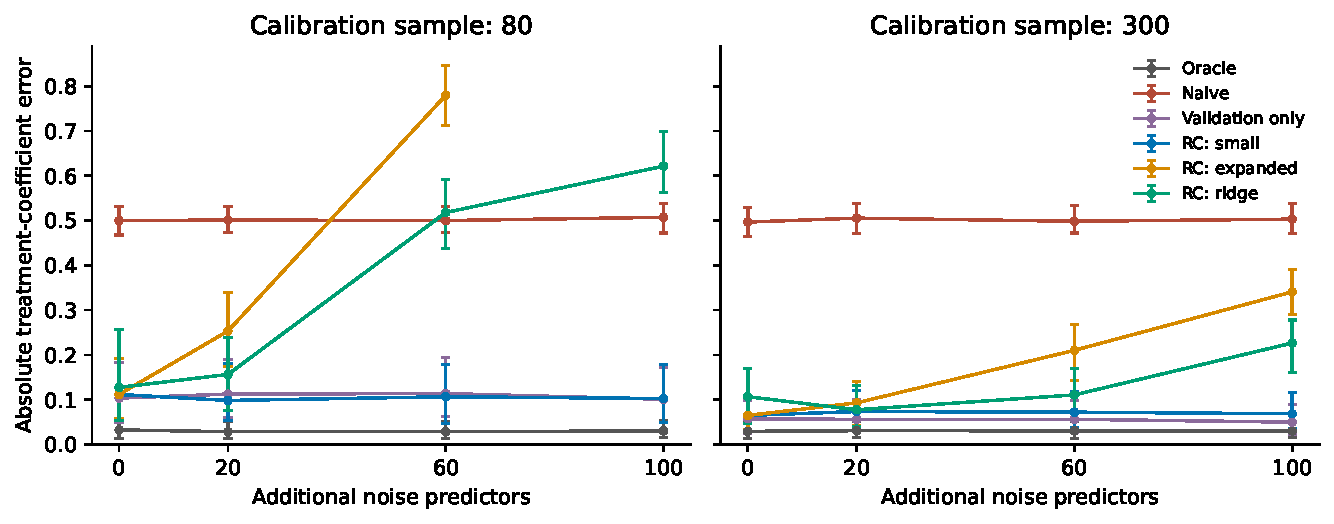
\includegraphics[width=\textwidth]{figures/dimension.pdf}
\caption{Treatment-coefficient error as calibration gains irrelevant predictors. Points show median absolute error; bars show the 25th--75th percentiles across replications, not confidence intervals or Monte Carlo standard errors. The expanded OLS curve stops where its calibration fit is nonunique. The oracle observes target labels and is an infeasible reference.}
\label{fig:dimension}
\end{figure}

For fixed-dimensional, regular calibration fits, inference must account for both samples. Resampling calibration and target observations independently and refitting both stages is an established solution \citep{boe2023}. The separate coverage experiment in Table~\ref{tab:coverage} compares that procedure with second-stage HC1 intervals for the small OLS calibration. It uses \InferenceReps{} replications and \BootstrapDraws{} bootstrap resamples per interval. Its conclusions are conditional on the frozen prediction model. A random training stage would require a corresponding uncertainty analysis. The experiment does not validate bootstrap inference after arbitrary regularization, model selection, or weak identification.

\section{Implications for practice}
Regression calibration offers a transparent starting point for machine-learned covariates when the target is a justified linear model. Start with all observed downstream regressors in the calibration span, verify that the calibrated covariates retain independent variation, and account for the labeled sample's estimation error. Assess target support separately from prediction fit. When the target is instead a population regression projection without the required exclusion restriction, or validation sampling supplies a different route to identification, moment-correction and design-based methods address a different problem.

For nonlinear outcome means, replacing a covariate by its conditional mean is generally an approximation; this limitation is also established \citep{carroll1990}. It is not a universal impossibility result. Logistic curvature changes sign, so Jensen's inequality does not give a global direction of bias. With a log mean and a conditionally Gaussian calibration residual of constant variance, integration can change only the intercept while preserving slopes \citep{wang2012}. The relevant comparison is therefore between assumptions, targets, and available information, rather than a blanket division between linear models that need calibration and nonlinear models that need something else.

The baseline's value is that its requirements are visible. It forces a proposed improvement to explain whether it reduces calibration error, relaxes an outcome restriction, transports information more credibly, or improves efficiency for the same estimand.

\paragraph{Replication and assistance.}
Code, generated results, and the simulation specification are available at
\url{https://github.com/finite-sample/calibration-baseline}.
The specification was written during revision after inspecting the previous design; it is not a preregistration. AI tools assisted with the literature audit, manuscript revision, code, and checks.

\begingroup
\small\singlespacing
\setlength{\bibsep}{3pt}
\bibliographystyle{apalike}
\bibliography{references}
\endgroup

\clearpage
\appendix
\renewcommand{\thetable}{A\arabic{table}}
\renewcommand{\thefigure}{A\arabic{figure}}
\renewcommand{\theequation}{A\arabic{equation}}
\setcounter{table}{0}\setcounter{figure}{0}\setcounter{equation}{0}
\section{Derivations and simulation details}

\subsection{Calibration and coefficient error}
Substitute $Y=R_m^\top\theta+(X-m)^\top\gamma+\varepsilon$ into the population OLS normal equations. Since $R_m$ is measurable with respect to $H$, exogeneity gives $\E_U[R_m\varepsilon]=0$. Therefore
\begin{equation}
Q_m\{\theta_U(m)-\theta\}=\E_U[R_m(X-m)^\top]\gamma.
\end{equation}
This proves both identities in the text. A conditional mean makes the matrix on the right zero. For a population projection onto $B$, each residual is orthogonal to every component of $B$. Since both $V$ and $m$ lie in that span, it is also zero. Neither argument guarantees nonsingularity of $Q_m$.

For consistency, condition on the calibration sample and use independence of target observations. Target $L_2$ convergence of $\widehat m$ to $m$ implies convergence of $\E_U[R_{\widehat m}R_{\widehat m}^\top]$ and $\E_U[R_{\widehat m}Y]$ by Cauchy--Schwarz, provided $Y$ has a finite second moment. Uniformly controlled fourth moments of the fitted regressors and $Y$ suffice for the corresponding triangular-array sample moments to converge as $n_u\to\infty$. Continuity of matrix inversion at nonsingular $Q_m$ gives consistency. This fixed-dimensional argument is a sufficient condition, not a rate theorem for high-dimensional calibration.

For scalar $X$ and a perturbation $m_t=m_0+t h$, where $m_0=\E_U[X\mid H]$, the derivative of the residual moment at zero is
\begin{equation}
\left.\frac{d}{dt}\E_U[R_{m_t}(X-m_t)]\right|_{t=0}
=-\E_U[R_{m_0}h].
\end{equation}
The derivative from changing $R$ vanishes by conditional-mean orthogonality; the displayed term generally does not. This establishes the first-order sensitivity of the ordinary plug-in.

\subsection{Omitted treatment and ridge shrinkage}
In the example, $\operatorname{Var}(D)=1$, $\operatorname{Var}(X)=2$, $\operatorname{Var}(W)=3$, and every covariance involving $D$ and either $X$ or $W$ equals 1; $\operatorname{Cov}(X,W)=2$. The population regression of $Y$ on $(D,W)$ has slopes $(1,1/2)$. Rescaling $W$ to $2W/3$ leaves the coefficient on $D$ equal to 1. Replacing $W$ by $(D+W)/2$ instead gives slopes $(1/2,1)$.

Write $X=D+v$ using the Gaussian conditional representation, where $v$ has variance 1 and is independent of $D$. Residualizing $W$ on $D$ leaves $v+u$, with variance 2. The standardized predictor is $(v+u)/\sqrt 2$. Penalized population regression of $v$ on this predictor has coefficient $1/[\sqrt 2(1+\lambda)]$. Hence $m_\lambda=(1-b)D+bW$, $b=1/[2(1+\lambda)]$. Substituting $W=(m_\lambda-(1-b)D)/b$ in the population projection $Y=D+W/2+\text{residual}$ gives
\begin{equation}
\beta_D(\lambda)=1-\frac{1-b}{2b}=\frac12-\lambda,
\qquad \gamma(\lambda)=\frac{1}{2b}=1+\lambda.
\end{equation}
An invertible affine prediction of $W$ does not change these arguments when the intercept is included and residual predictors are standardized.

\subsection{Transport of a restricted projection}
Let $V=1$ and $X=H^2$, with $H\sim\operatorname{Uniform}[0,1]$ in calibration and density $2h$ on the same interval in the target population. Both populations have exactly the same conditional mean and support. In calibration, the linear projection of $X$ on $(1,H)$ is $m_C=H-1/6$. In the target population, $\E_U[X]=1/2$ and $\E_U[m_C]=2/3-1/6=1/2$, but
\begin{equation}
\E_U[m_C(X-m_C)]=\frac{1}{90}\ne0.
\end{equation}
Indeed, $\operatorname{Cov}_U(H,H^2)=1/15$ and $\operatorname{Var}_U(H)=1/18$. If $Y=X$, target OLS of $Y$ on $(1,m_C)$ has slope $6/5$, rather than 1. Estimating the target conditional mean $H^2$ or a target-weighted linear projection repairs this particular example. Stable conditional means and common support alone do not transport a restricted projection's orthogonality.

\subsection{A support gap that more labels cannot close}
Suppose labeled $H$ is uniform on $[0,1]$ and target $H$ is uniform on $[0,2]$. Consider $X=m_j(H)$, with $m_0(h)=h$ and $m_1(h)=h+(h-1)_+$. The two worlds give identical distributions for calibration labels and target predictors. For any predictor $a(h)$ learned solely from these inputs,
\begin{equation}
\frac{(a-m_0)^2+(a-m_1)^2}{2}
\geq\frac{(m_1-m_0)^2}{4}.
\end{equation}
Integrating over target $H$ gives average risk at least $1/24$, so at least one world has target MSE at least $1/24$, even with infinitely many calibration observations. The inequality also holds after averaging over any fitting randomness. Both candidate means are continuous. Additional structural restrictions, labels outside the original support, or an informative outcome model can change the conclusion. This example establishes a limit on learning calibration from the stated inputs, not a general impossibility of downstream inference.

\subsection{Simulation specification and reporting}
The frozen learner is scikit-learn ridge with penalty 1 in its sum-of-squares convention and an intercept, trained on 1,000 observations. The calibration ridge penalty is instead 0.1 in a mean-squared-loss convention, with intercept and treatment unpenalized. Calibration-only residualization and scaling are applied to target features; no target labels enter a feasible estimator. Independent pseudo-random streams index each sample-size, dimension, and replication cell. The generator, seeds, versions, and frozen prediction coefficients are recorded in \texttt{results/metadata.json}; replicate-level results are in \texttt{results/replications.jsonl}.

The primary summaries are the median signed error, median absolute error, and absolute-error quartiles. Run RMSE is the square root of the average squared error among the realized replications; it is descriptive, not an estimate accompanied by a normal-theory Monte Carlo interval. All methods share samples within a replication. Coverage MC SE is $\sqrt{\widehat p(1-\widehat p)/R}$. Unexpected errors stop execution; rank failures are counted without substituting coefficients.

This reporting choice matters even in the simple Gaussian design. Write small fitted calibration as $\widehat m=\widehat a_0+\widehat a D+\widehat b W$, and target OLS of $Y$ on $(D,W)$ as having slopes $(\widehat d,\widehat c)$. The calibrated treatment estimate is $\widehat d-\widehat c\widehat a/\widehat b$. Conditional on a full-rank calibration design, $(\widehat a,\widehat b)$ is nondegenerate normal. Its density at $\widehat b=0$ is positive, and the conditional second moment of $\widehat a$ there is positive. Target data are independent, with $\widehat c\ne0$ almost surely. The resulting ratio has infinite second moment. Rare draws near zero can dominate squared error even though none appears in a modest simulation. Fixed-dimensional consistency and local asymptotic normality at a nonzero population slope do not imply finite moments at every sample size. The initial replacement design used RMSE error bars; mathematical review after its first run prompted the change to quantiles recorded in \texttt{analysis\_plan.json}. No observations or replications were trimmed.

\begin{table}[htbp]\centering\small
\caption{Calibration complexity and treatment-coefficient error.}
\label{tab:dimension}
\begin{tabular}{rrlrrrr}\toprule
$n_c$ & $q$ & Method & Median error & Run RMSE & $X$ MSE & Failed \\\midrule
80 & 0 & Oracle & -0.001 & 0.044 & 0.000 & 0 \\
80 & 0 & Naive & 0.500 & 0.500 & 0.668 & 0 \\
80 & 0 & Validation only & -0.003 & 0.160 & --- & 0 \\
80 & 0 & RC: small & -0.001 & 0.173 & 0.523 & 0 \\
80 & 0 & RC: ridge & -0.104 & 0.229 & 0.526 & 0 \\
80 & 100 & RC: small & 0.001 & 0.163 & 0.520 & 0 \\
80 & 100 & RC: expanded & --- & --- & --- & 400 \\
80 & 100 & RC: ridge & 0.621 & 0.634 & 1.240 & 0 \\
300 & 0 & Oracle & -0.003 & 0.044 & 0.000 & 0 \\
300 & 0 & Naive & 0.497 & 0.501 & 0.668 & 0 \\
300 & 0 & Validation only & -0.004 & 0.086 & --- & 0 \\
300 & 0 & RC: small & 0.001 & 0.092 & 0.505 & 0 \\
300 & 0 & RC: ridge & -0.101 & 0.142 & 0.508 & 0 \\
300 & 100 & RC: small & 0.003 & 0.097 & 0.505 & 0 \\
300 & 100 & RC: expanded & 0.341 & 0.349 & 0.761 & 0 \\
300 & 100 & RC: ridge & 0.226 & 0.239 & 0.691 & 0 \\
\bottomrule\end{tabular}
\par\smallskip\begin{minipage}{0.96\textwidth}\footnotesize
Each cell uses 400 independent replications. The full grid is in the replication files. At $q=0$, expanded OLS equals small RC. $q$ counts added calibration predictors; the downstream regression always contains an intercept, treatment, and one true, predicted, or calibrated covariate. $X$ MSE is evaluated on target observations. Validation-only OLS makes no imputation. Failed denotes nonunique OLS fits; no pseudoinverse coefficient is substituted. Oracle OLS uses target labels unavailable to the feasible methods. Run RMSE is descriptive: small OLS calibration has infinite finite-sample population MSE in this design.
\end{minipage}\end{table}

\begin{table}[htbp]\centering\small
\caption{Uncertainty from estimating the small calibration model.}
\label{tab:coverage}
\begin{tabular}{rlrrr}\toprule
$n_c$ & Interval & Coverage & MC SE & Mean width \\\midrule
80 & Second stage HC1 & 0.580 & 0.025 & 0.265 \\
80 & Two-sample bootstrap & 0.932 & 0.013 & 0.635 \\
300 & Second stage HC1 & 0.825 & 0.019 & 0.263 \\
300 & Two-sample bootstrap & 0.940 & 0.012 & 0.384 \\
\bottomrule\end{tabular}
\par\smallskip\begin{minipage}{0.96\textwidth}\footnotesize
Nominal coverage is 0.95; 400 independent replications and 399 resamples per bootstrap interval. Both samples are independently resampled and both regressions refit. Second-stage HC1 treats estimated calibration as fixed. No fits failed. These results concern only the fixed, three-parameter OLS calibration.
\end{minipage}\end{table}

\end{document}
